\documentclass[a4paper]{article}

\usepackage{amsmath}
\usepackage{listings}
\usepackage{amsfonts}
\usepackage{amssymb}
\usepackage{graphicx}
\usepackage{titling}
\usepackage[utf8]{inputenc}
\usepackage[english]{babel}
\usepackage{fancyhdr}
\usepackage{lastpage}
\usepackage{textcomp}
\usepackage{hyperref}
\usepackage{float}

\addtolength{\oddsidemargin}{-.875in}
\addtolength{\evensidemargin}{-.875in}
\addtolength{\textwidth}{1.75in}
\addtolength{\topmargin}{-.875in}
\addtolength{\textheight}{1.75in}

\title{\Huge Medical Technologies Synopsis \vspace{1cm}}
\author{MrRattoSpaccio, Lolinear}
\date{May 23rd 2019}
\setcounter{page}{0}
\pagestyle{fancy}
\fancyhf{}

\fancyfoot[C]{Page \thepage \hspace{1pt} of \pageref{LastPage}}

\begin{document}
\maketitle
\thispagestyle{empty}
\pagebreak
\tableofcontents

\section{Introduction}
\subsection{Tipologie di Ingegneri biomedici}
\begin{description}
    \item[Clinici] Lavorano negli ospedali, essi aiutano altri operatori degli
    ospedali a scegliere l'apparecchiatura più giusta per l'assistenza ai 
    pazienti. Si occupano anche di assicurare che le apparecchiature siano
    sicure ed affidabili.
    \item[Progetto e Ricerca] Lavorano nelle grandi aziente, progettano sistemi
    per il monitoraggio continuo dei pazienti critici, organi artificiali, o 
    schemi e procedure per somministrare terapie in modo sicuro ed efficace.ù
    \item[Riabilitazione] Utilizzano la tecnologia ed i calcolatori per 
    aiutare le persone con disabilità e migliorare la qualità della loro vita.
    \item[Ricerca (Scuole)] Lavorano nei laboratori di ricerca di scuole di 
    medicina o università, acquisendo nuove conoscenze sugli organismi viventi.
    \item[Vari] Alcuni studiano cellule ed insiemi di molecole, alcuni organi
    composti da insiemi di cellule, altri creano modelli matematici che 
    descrivono le funzionalità del corpo. Altri ancora studiano materiali
    artificiali necessari alla creazione di dispositivi medicali. 
\end{description}
\subsection{Dispositivi medicali (DM)}
\subsubsection{Definizione}
\paragraph{Completa}
S’intende per dispositivo medicale, qualunque strumento, apparecchio, 
apparecchiatura, materiale, prodotto, all’eccezione dei prodotti d’origine 
umana, o altro articolo usato da solo o in combinazione, compresi gli accessori
e software necessari per il suo funzionamento, destinato dal fabbricante ad 
essere impiegato sull'uomo per scopi medici e la cui azione principale voluta 
non si ottiene con mezzi farmacologici o immunologici o metabolici, ma dove 
la funzione può essere assistita da tali mezzi.
\paragraph{Concisa}
Ogni prodotto utilizzato per scopi medici che non è, né un medicamento, né un 
prodotto biologico, è identificabile con la terminologia di Dispositivo Medico.
\subsubsection{Utilizzi}
\begin{itemize}
    \item Diagnosi, prevenzione, controllo, terapia o attenuazione di una 
    malattia
    \item Diagnosi, controllo, terapia, attenuazione o compensazione di una 
    ferita o di un handicap
    \item Studio, sostituzione o modifica dell'anatomia o di un processo 
    fisiologico
    \item Controllo e gestione del concepimento
\end{itemize}
\subsubsection{Categorie}
\begin{description}
    \item[Impiantabili attivi (DMIA)] Pacemaker, defibrillatori, pompe 
    \item[Diagnostica in Vitro (DM DIV)] Reagenti per le diagnosi
    \item[Compensazione degli handicap] Sedia a rotelle, apparecchi acustici
    occhiali, ecc.
    \item[Su misura] protesi dentarie, plantari ortopedici, ecc.
    \item[Diagnostica/Pratiche Terapeutiche/Supporto Vitale] Scanner, macchina
    per la dialisi, radioterapia, monitor di sorveglianza, defibrillatori
    esterni
    \item[Monouso] Aghi, bende, siringe, ecc.
    \item[Impianti chirurgici non attivi] protesi d'anca, valvole cardiache, ecc.
\end{description}
\subsection{Dispositivi Medicali Impiantabili Attivi (DMIA)}
Dispositivi medici che sono progettati per essere impiantati totalmente o in 
parte nel corpo umano... e che dipendono per il loro corretto funzionamento 
da una fonte d’energia elettrica o da qualsiasi altra fonte d’energia diversa 
da quella prodotta direttamente dal corpo umano o dalla gravità.
\subsection{Dispositivi Medicali di Diagnostica In Vitro (DM DIV)}
Prodotti, reagenti, materiali, strumenti... destinati ad essere utilizzati in 
vitro per l'esame di campioni provenienti dal corpo umano con lo scopo di 
fornire informazioni relative a una condizione fisiologica o patologica.
\subsection{Classificazione dei DM}
I dispositivi medici, eccetto i DMIA e i DM DIV sono classificati in 4 classi:
\begin{itemize}
    \item Classe I $\to$ Rischio potenziale debole (Lenti da vista, 
    Stetoscopi, ecc.)
    \item Classe IIa $\to$ Rischio potenziale moderato (Lenti a contatto, 
    Catateri urinari, ecc.)
    \item Classe IIb $\to$ Rischio potenziale elevato (Laser chirurgici, 
    Cemento osseo, ecc.)
    \item Classe III $\to$ Rischio potenziale critico (Stent, valvole cardiache, 
    ecc.)
\end{itemize}
Tutti i DMIA sono classificati come Classe III.
\subsubsection{Regole di classificazione}
\begin{itemize}
\item Il periodo d’utilizzo o più precisamente la durata in cui il dispositivo
è in continuità in contatto col paziente
\item L’invasività: il dispositivo è invasivo o no, e se lo è, qual è il grado
d’invasività (penetrazione attraverso un orifizio del corpo o tramite 
impianto chirurgico)
\item La possibilità o meno di riutilizzo
\item L’obiettivo terapeutico o diagnostico
\item La dipendenza da una fonte d’alimentazione diversa da quella umana
\item La parte del corpo che viene a contatto con il dispositivo medico: sistema circolatorio centrale,
sistema nervoso centrale, ecc.
\end{itemize}
\paragraph{Classe I}
Strumenti chirurgici riutilizzabili, dispositivi medici non invasivi, 
dispositivi medici invasivi per uso temporaneo, ecc.
\paragraph{Classe IIa}
Dispositivi medici di classe I sterili e/o con funzione di misurazione, lenti a 
contatto, protesi dentarie, ecc.
\paragraph{Classe IIb}
Dispositivi medici impiantabili a lungo termine, ecc.
\paragraph{Classe III}
Dispositivi medici impiantabili a lungo termine in contatto con il cuore, il 
sistema circolatorio centrale o il sistema nervoso centrale, i dispositivi 
medici impiantabili riassorbibili, protesi al seno, protesi d'anca, protesi
di ginocchio, ecc.
\subsection{Prodotti di Frontiera}
Si parla di prodotti combinati o di frontiera:
\begin{itemize}
    \item Quando un DM forma con un farmaco un prodotto un prodotto integrato.
    Ad esempio le siringhe pre-riempite.
    \item Quando un DM incorpora una sostanza che, utilizzata sola, può essere
    considerata come un farmaco. Ad esempio il cemento osseo con antibiotico.
\end{itemize}
Il prodotto combinato è considerato come un farmaco o un dispositivo medico in 
base all'azione principiale prevista.
\subsection{Considerazioni e Prospettive nel campo}
Troppo spesso l'utilizzo delle tecnologie medicali o viene promosso con
eccessiva facilità senza averne valutato adeguatamente le implicazioni o viene 
limitato dai timori derivanti dall’incertezza circa gli esiti e le conseguenze
del loro impiego. \\
La figura tecnica di riferimento per le tecnologie sanitarie, quale l’ingegnere 
biomedico, deve compiere uno sforzo di ampliamento del suo background formativo
e focalizzare maggiore attenzione sugli aspetti di valutazione dei rischi, dei 
costi e dei benefici delle nuove tecnologie sanitarie.

\section{Organizzazione del corpo umano, cellule e tessuti}
\paragraph{Anatomia} La scienza che studia la struttura di un corpo e le 
relazioni tra le sue parti.
\paragraph{Fisiologia} La scienza che studia come funzionano le parti di un
organismo.
\subsection{Livelli di organizzazione ed apparati del corpo}
\begin{enumerate}
    \item Livello della chimica (o molecolare): include gli atomi e le molecole
    \item Livello cellulare: le cellule sono le unità strutturali e funzionali 
    di base dell’organismo
    \item Livello dei tessuti: i tessuti sono costituiti da gruppi di cellule 
    che svolgono una funzione particolare
    \item Livello degli organi: i diversi tipi di tessuti si uniscono a formare 
    gli organi
    \item Livello dei sistemi e degli apparati: i sistemi sono costituiti da 
    organi con la medesima origine embriologica; gli apparati possono avere 
    struttura o derivazione embriologica diversa
    \item Livello dell’organismo
\end{enumerate}
\begin{figure}[H]
    \centering
    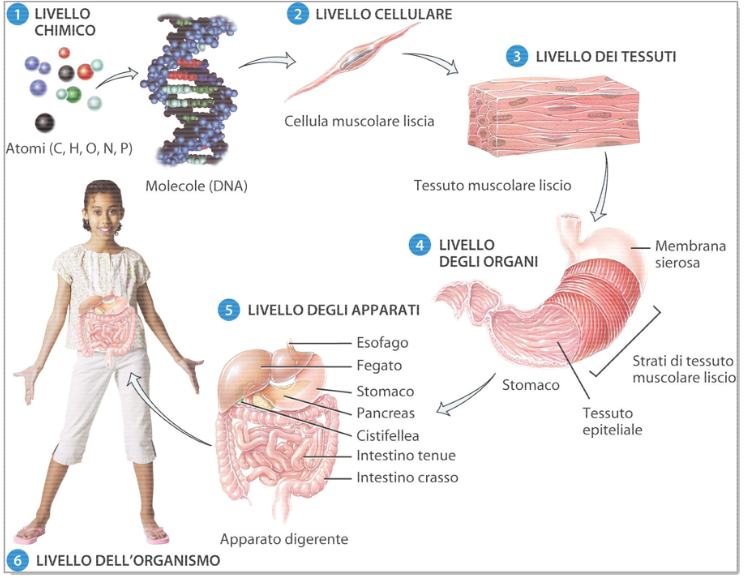
\includegraphics[scale=0.3]{figures/levels.png}
    \caption{Livelli di organizzazione}
\end{figure}
\subsection{Processi della vita}
\begin{description}
    \item[Metabolismo] L'insieme di tutti i processi chimici che avvengono nel
    corpo, tra cui la scissione di molecole e la loro sintesi
    \item[Reattività] La capacità di rilevare e di rispondere ai cambiamenti
    dell'ambiente interno/esterno
    \item[Movimento] Gli spostamenti di tutto il corpo, compresi gli organi, le
    cellule e gli organuli cellulari
    \item[Accrescimento] L'aumento delle dimensioni corporee
    \item[Differenziazione] Il processo in cui le celle indifferenziate si
    specializzano
    \item[Riproduzione] Intesa come sintesi di nuove cellule e generazione di
    un nuovo individuo
\end{description}
\subsection{Omeostasi}
L'omeostasi è il mantenimento della stabilità delle condizioni del corpo. 
Essa:
\begin{itemize}
    \item Garantisce il funzionamento cellulare
    \item Interviene per ripristinare le condizioni di stabilità 
    controbilanciando i cambiamenti interni/esterni
    \item Varia entro un ristretto ambito compatibile coi processi vitali delle
    cellule
\end{itemize}
Esistono dei sistemi di feed-back che permettono il mantenimento dell'omeostasi,
rappresentati da un ciclo di eventi dove la condizione del corpo viene 
continuamente monitorata, valutata e modificata. Così facendo si ottiene una
condizione controllata, perturbabile da uno \textbf{stimolo}.

\subsubsection{Sistemi di feed-back}
Un sistema di feed-back è costituito da:
\begin{description}
    \item[Recettore] Struttura che rileva i cambiamenti che avvengono in una 
    condizione controllata e invia tale informazione o input a un centro di 
    controllo
    \item[Centro di controllo] Valuta l’input ricevuto e invia comandi in 
    uscita all’effettore per il ripristino della condizione controllata
    \item[Effettore] Struttura che riceve l’output e produce una risposta 
    che modifica la condizione controllata
\end{description}
\end{document}